\chapter{Implementacja symulatora w środowisku przeglądarki internetowej}
\label{cha:implementacja}

Niniejszy rozdział omawia najważniejsze zagadnienia związane z implementacją
symulatora \en w środowisku przeglądarki internetowej. Podstawową technologią
użytą do stworzenia aplikacji był natywny dla przeglądarek język \js.
Symulator nie jest zależny od żadnego rozszerzenia czy też dodatku do
przeglądarki, aby nie ograniczyć dostępu do aplikacji użytkownikom, którzy
mogą nie mieć możliwości instalacji takich komponentów (choćby ze względu na
brak uprawnień lub wiedzy). Głównymi założeniami projektowymi implementacji
było zniwelowanie wad wymagającego środowiska przeglądarki internetowej oraz
optymalne wykorzystanie jego zalet.

\section{Język programowania -- JavaScript}

Środowisko przeglądarki internetowej oraz \js nie były w zamierzeniu tworzone
z myślą o dużych, złożonych aplikacjach. Przeciwnie, język \js miał być
językiem wyjątkowo prostym, łatwym do nauczenia, odpornym na błędy i
przeznaczonym głównie do tworzenia prostych skryptów wzbogacających treść
stron internetowych. Jednak gwałtowny rozwój technologii internetowych
diametralnie zmienił tę sytuację. Aplikacje dostępne przez przeglądarkę stały
się zaawansowane i złożone, często wypierając swoje odpowiedniki instalowane
bezpośrednio na komputerach użytkowników. Jednak sama technologia niewiele się
zmieniła od swojego powstania. Pierwsza specyfikacja \ow{ECMAScript}
(definiująca i standaryzująca język \ow{JavaScript}) pojawiła się w roku 1997,
została uaktualniona również w latach 1998 oraz 1999, a przez następnych
dziesięć lat, aż do roku 2009, nie uległa żadnym zmianom. Dziesięć lat dla
takiej technologii stanowi ogromny zastój, szczególnie iż przypadł na okres
wyjątkowo dynamicznego rozwoju aplikacji internetowych. Obrazuje to fakt, iż
sam rozwój języka często nie nadążał za jego zaawansowanymi zastosowaniami.

W związku z tą sytuacją, tworząc złożone aplikacje w języku \js, programiści
mogą napotkać wiele trudności. Brakuje dostępu do rozwiązań, które często
uznawane są za podstawowe i niezbędne. Różne są też koncepcje i podejścia do
zagadnień takich jak programowanie obiektowe czy rozwiązywanie zależności.
Jednak należy podkreślić, że przy tym przeglądarka internetowa i \js stanowią
doskonałe środowisko uruchomieniowe dla aplikacji. Przeglądarka stanowi dziś
podstawowe oprogramowanie praktycznie każdego komputera. Aplikacje napisane w
języku \js są z natury wieloplatformowe, gdyż wykonywane przez interpreter. Co
więcej, przez wieloplatformowość można rozumieć nie tylko różne systemy
operacyjne komputerów osobistych ale także urządzenia mobilne, które również
posiadają zaawansowane przeglądarki. Aplikacje \js nie wymagają również od
użytkownika instalacji, uprawnień administratora, a aktualizacje są niezwykle
łatwe do przeprowadzenia. Jest to potencjał, który zdecydowanie jest wart
poradzenia sobie z problemami wymienionymi wcześniej. Szczególnie dla aplikacji
edukacyjnej, która musi być łatwo dostępna dla jak najszerszego grona odbiorców.

\js nie narzuca żadnego stylu programowania. Jest on językiem skryptowym,
zorientowanym obiektowo lecz o prototypowym modelu dziedziczenia. Ponadto jest
dynamiczny, słabo typowany, a funkcje są obiektami pierwszoklasowymi. Doskonale
wspiera wiele paradygmatów programowania, takich jak programowanie zorientowane
obiektowo, imperatywne czy też funkcyjne.

W związku z tym twórcy aplikacji mają bardzo dużą dawkę elastyczności w
podejściu do strukturyzacji swojej pracy. Nic nie jest z góry narzucone i
możliwe jest skorzystanie ze wszystkich cech języka w zależności od potrzeb.
Jednak ta elastyczność również może stanowić przyczynę tworzenia aplikacji
nieczytelnych, nieustrukturyzowanych, w sposób chaotyczny mieszających różne
paradygmaty i wzorce. Czyli aplikacji trudnych w rozwoju oraz utrzymaniu.
Dlatego też możliwości \js powinny być stosowane z pełną świadomością korzyści i
konsekwencji. Natomiast architektura aplikacji powinna się opierać na solidnych,
sprawdzonych wzorcach, aby minimalizować omówione powyżej ryzyko.

\section{Architektura systemu -- wzorzec Model--View--Controller}

Na etapie projektowania symulatora \en zostały wyodrębnione dwa główne zadania,
które miały być realizowane przez aplikację:
\begin{itemize}
\item Obliczenia fizyczne.
\item Wizualizacja.
\end{itemize}

Zarówno silniki fizyczne wraz z potrzebnymi modelami danych jak i metody
wizualizacji wymagają dość złożonych algorytmów. Oczywistym stało się, że
należy starać się stworzyć jak najbardziej niezależne moduły odpowiedzialne za
realizację każdego z tych zadań. Jest to możliwe -- wizualizacja oczywiście
musi korzystać z wyników obliczeń fizycznych, jednak same silniki fizyczne nie
muszą nic wiedzieć o fakcie istnienia wizualizacji, ani być bezpośrednio z
nimi związane. Umożliwiło to wprowadzenie jasnego podziału na luźno powiązane
grupy komponentów, które realizują dwa wymienione wcześniej cele.

Uwzględniając powyższe obserwacje, ostateczna architektura aplikacji powstała na
bazie wzorca projektowego \emph{Model-View-Controller}. Schemat ideowy systemu
\en przedstawia rysunek \ref{fig:architektura}. Użyty wzorzec projektowy jest
powszechnie stosowany w aplikacjach, które posiadają graficzny interfejs
użytkownika. Skupia się na oddzieleniu logiki biznesowej oraz model danych od
ich reprezentacji. Ujmując to ogólniej, zapewnia rozdzielenie obowiązków (ang.
Separation of
Concerns\footnote{\url{http://en.wikipedia.org/wiki/Separation_of_concerns}}).
Wpisuje się to doskonale we wspomniane powyżej potrzeby symulatora \en, dlatego
też właśnie ten wzorzec został użyty jako podstawa architektury.

Wyraźny podział funkcjonalności przyniósł wiele korzyści, z których
najważniejsze to:

\begin{itemize}
\item Czytelna, jasna organizacja kodu.

\item Łatwe utrzymanie aplikacji.

\item Niepowiązane, samodzielne obiekty, które realizują zadania ogólne i mogą
być ponownie użyte (np. większość wizualizacji).

\item Brak związania silników fizycznych z przeglądarką internetową. Wynika to
właśnie z oddzielenia od warstwy prezentacji. Dzięki temu możliwe jest użycie
efektywnych testów zautomatyzowanych. Ta kwestia jest omówiona szerzej w sekcji
\ref{sec:zgodNode.js}.

\end{itemize}

Ponadto, należy podkreślić, iż architektura \en skupia się na stworzeniu grupy
jak najbardziej niezależnych obiektów i modułów, które są ze sobą powiązane
czytelną siecią zależności oraz realizują jasno określone zadania.

\begin{figure}[!h]
\centering
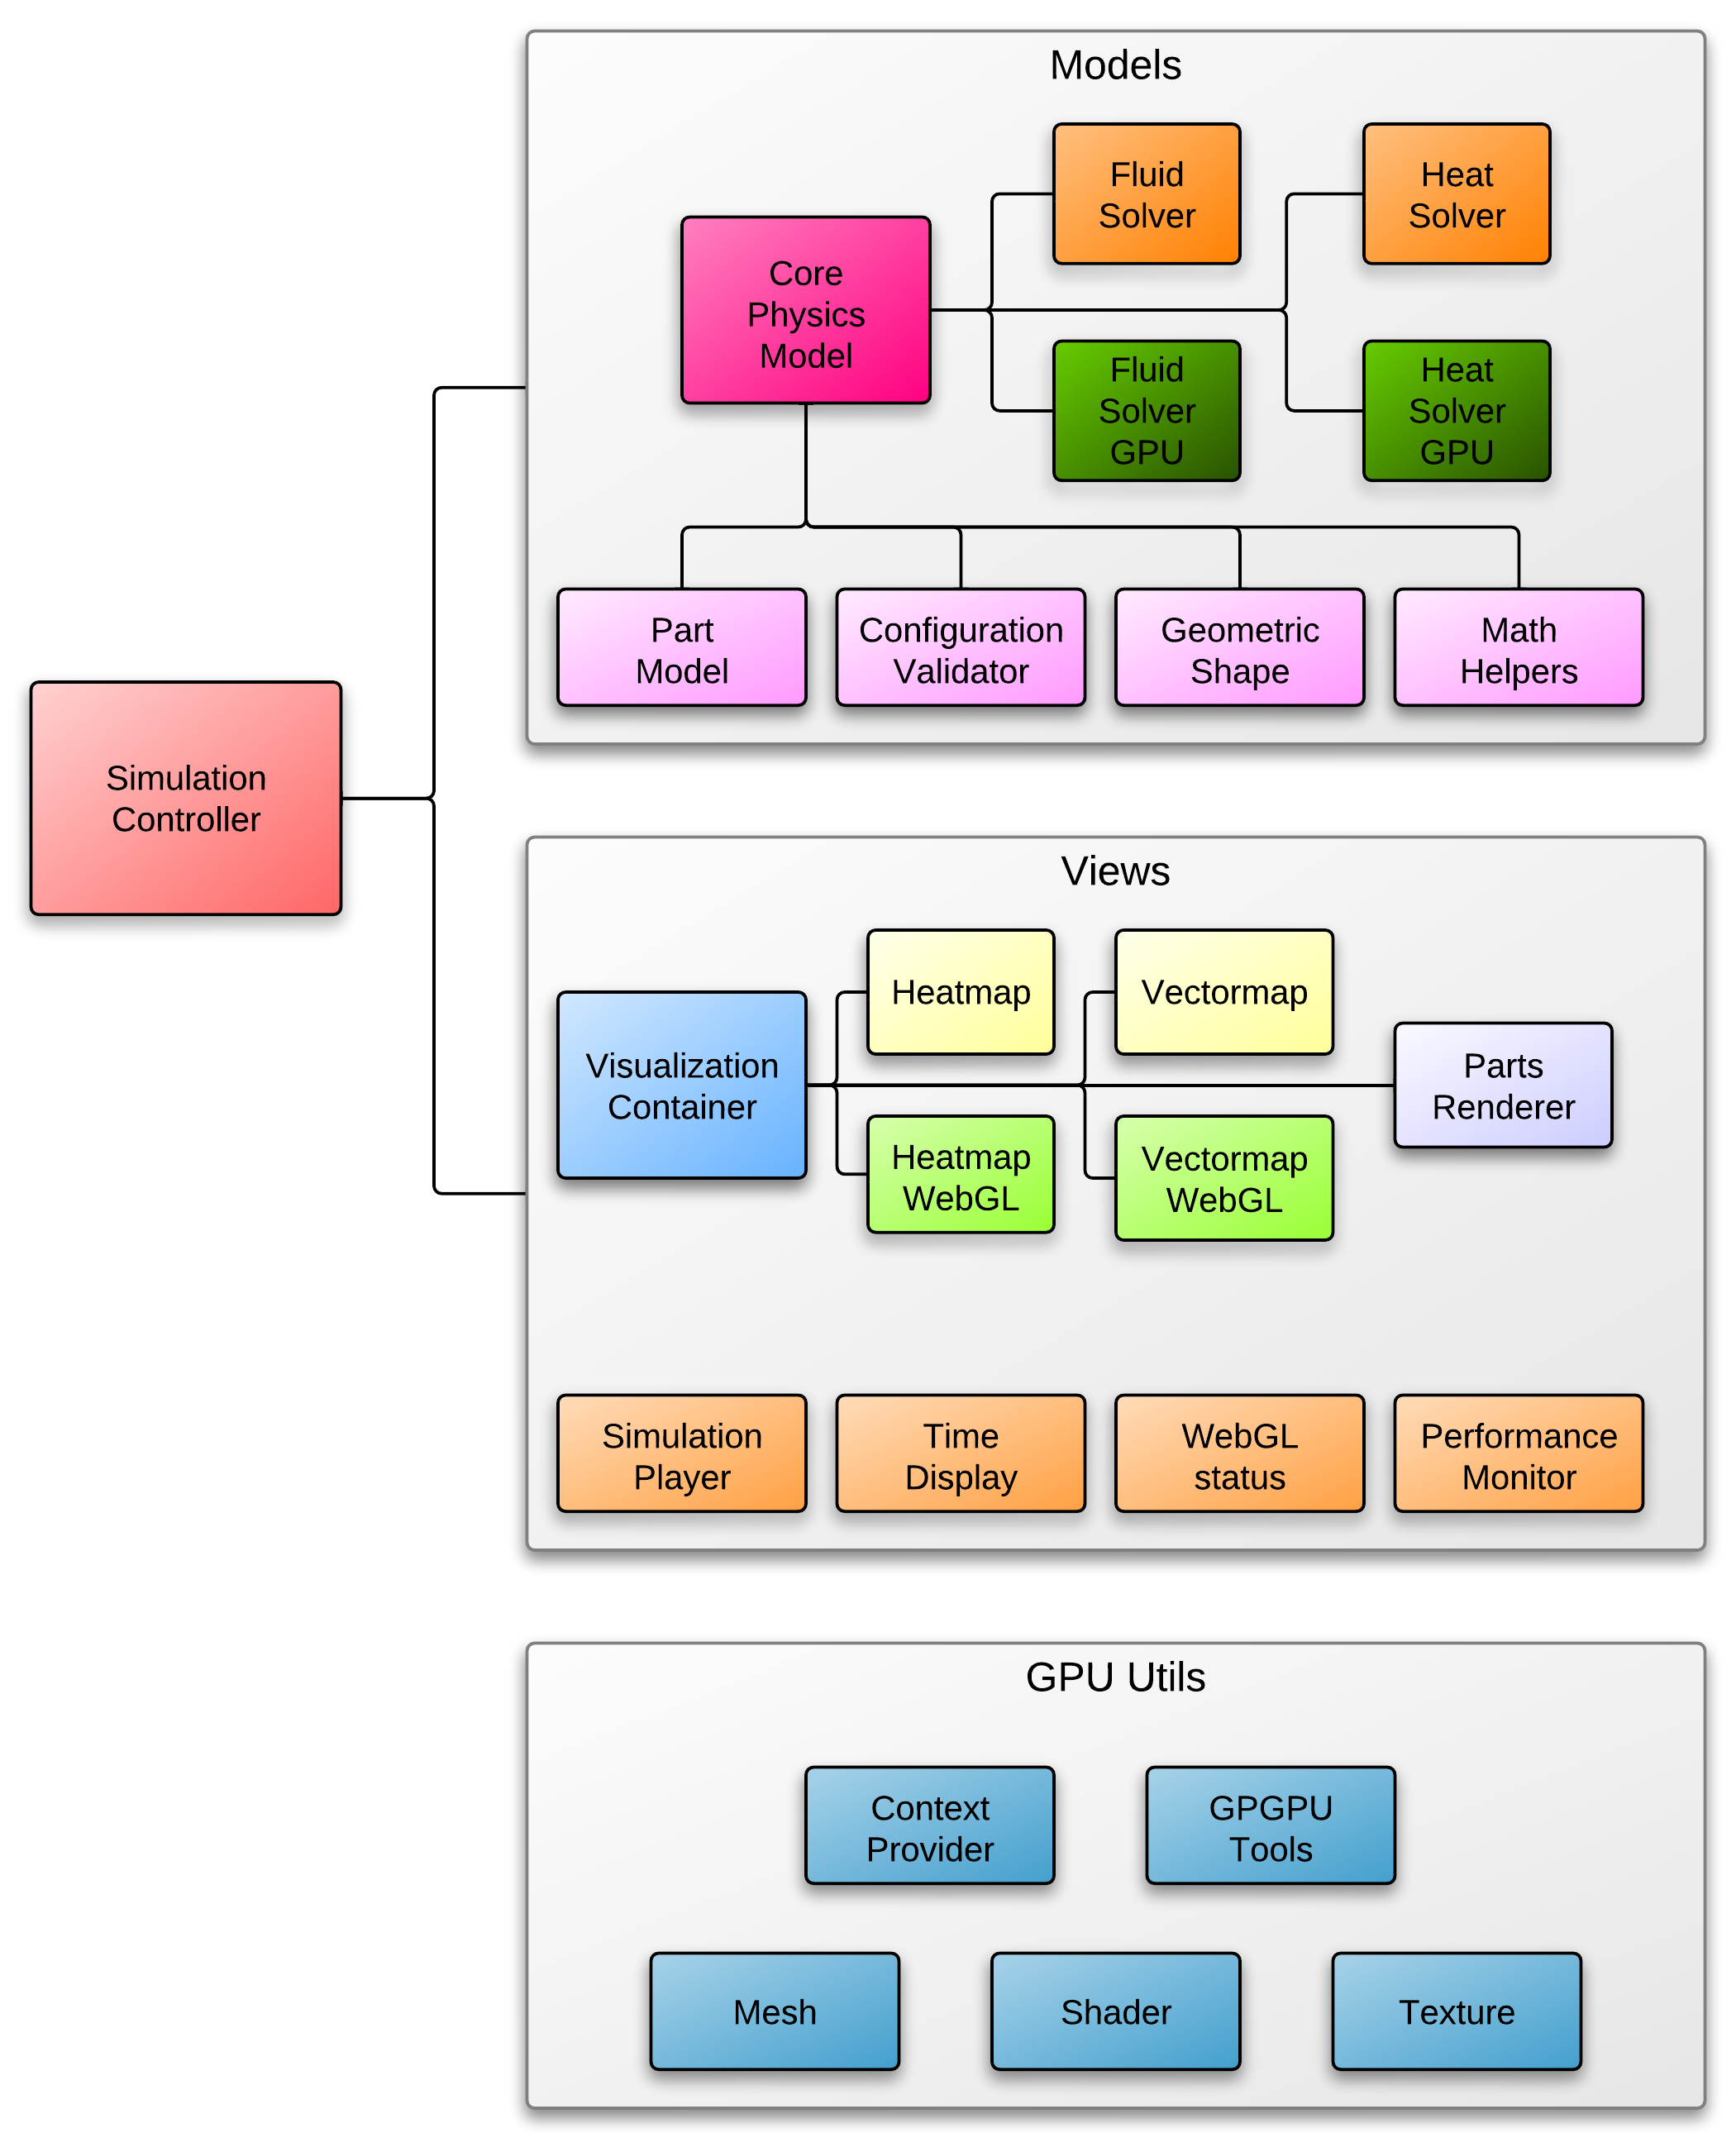
\includegraphics[width=\textwidth]{img/architektura}
\caption{Schemat ideowy architektury symulatora \en}
\label{fig:architektura}
\end{figure}

\section{Przegląd najistotniejszych jednostek symulatora}

W strukturze aplikacji można wyróżnić kilka wyraźnych grup charakteryzujących
się odmiennymi celami zasadniczymi. Wizualizacje tej struktury przedstawia
rysunek \ref{fig:architektura}, a kolejne sekcje przybliżają poszczególne grupy
oraz ich najważniejsze składniki.

\subsection{Modele}
\label{sec:modele}

Jest to zbiór obiektów odpowiedzialnych za przechowywanie i manipulowanie danymi
aplikacji. To właśnie w tej grupie znajdują się kluczowe dla całej aplikacji
silniki fizyczne odpowiadające za symulację przewodnictwa cieplnego oraz
dynamiki płynów.

\begin{description}

\item[Core Physics Model] tworzy i zarządza wszystkimi niezbędnymi dla obliczeń
fizycznych danymi. Można do nich zaliczyć siatki symulacyjne (reprezentowane
przez tablice \js bądź też dwuwymiarowe tekstury \ow{WebGL}) oraz zestaw
parametrów charakteryzujących warunki początkowe symulacji. Parametry te są
definiowane przez specjalny plik konfiguracyjny w formacie \ow{JSON}, dlatego
też można stworzyć bardzo wiele przypadków modelujących różnorakie zjawiska
fizyczne. Do zarządzania konfiguracją wykorzystywany jest jeden z pomocniczych
obiektów \textbf{Configration Validator}. Obliczenia fizyczne nie są
przeprowadzane przez sam obiekt \emph{Core Physics Model}. Deleguje on te
zadania do innych obiektów, tym samym realizując wzorzec projektowy strategii.

\item[Heat Solver oraz Fluid Solver] to obiekty implementujące algorytmy
fizyczne przewodnictwa cieplnego oraz dynamiki płynów przedstawione w sekcji
\ref{sec:silnikiFizyczne}. Implementacja została przeprowadzona wyłącznie w
języku \js dlatego też obliczenia wykonywane są na procesorze głównym
komputera.

\item[Heat Solver GPU oraz Fluid Solver GPU] to odpowiedniki obiektów
przedstawionych powyżej, jednak implementujące algorytmy fizyczne przy
wykorzystaniu technologii \ow{WebGL}. Stąd, główne obliczenia wykonywane są na
procesorze karty graficznej. Zapewnia to wielokrotnie lepszą wydajność.
Jednak, jako iż \ow{WebGL} jest technologią dość nową, obiekty te implementują
identyczną logikę jak wersje bazowe i są używane wyłącznie jeżeli konfiguracja
użytkownika spełnia odpowiednie wymagania.

\item[Part Model] to obiekt reprezentujący element symulacji nie będący płynem
(cieczą lub gazem). Dzięki obecności takich obiektów, możliwe jest stworzenie
ciekawych warunków początkowych odzwierciedlających rzeczywistość.  Zadaniem
elementów stałych symulacji jest tworzenie barier przepływu dla płynów. Ponadto,
elementy stałe symulacji mogą przewodzić ciepło co dodatkowo wzbogaca symulacje
i pozwala zaprezentować np. efekt wpływu pojemności cieplnej na zdolność
przewodzenia ciepła.

\item[Geometric Shape oraz Math Helpers] to obiekty pomocnicze, wykorzystywane
głównie przez obiekty \emph{Part Model}. Definiują różne reguły matematyczne
pomocne przy reprezentowaniu i wizualizowaniu kształtów geometrycznych.

\end{description}

\subsection{Widoki}

Jest to zbiór obiektów odpowiedzialnych za aspekt wizualny symulacji. Ich
głównym zadaniem jest wizualizacja czyli prezentowanie przedstawionych powyżej
modeli. Przykładowy zrzut ekranu aplikacji \en wraz z zaznaczonymi obszarami
wygenerowanymi przez poszczególne widoki prezentuje rysunek \ref{fig:widoki}.

\begin{figure}[!h]
\centering
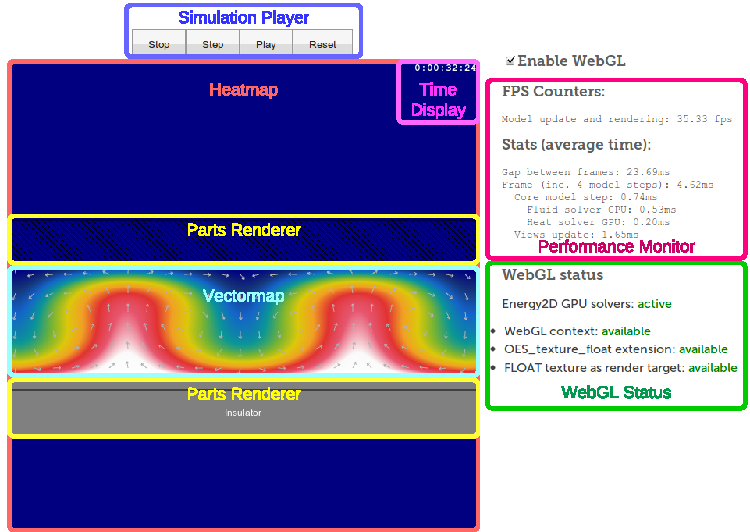
\includegraphics[width=\textwidth]{img/views}
\caption{Prezentacja poszczególnych widoków aplikacji \en}
\label{fig:widoki}
\end{figure}

\begin{description}

\item[Heatmap] to jeden z najważniejszych widoków, gdyż jest odpowiedzialny
za wizualizację temperatury. To dzięki temu możliwe jest obserwowanie zjawisk
zachodzących podczas symulacji. Wzorowany jest na obrazie kamer termowizyjnych.
Dostępnych jest także kilka palet kolorów.

\item[Vectormap] to widok odpowiedzialny za wyświetlanie strzałek prezentujących
prędkość i kierunek przepływu płynu. Umożliwia to lepsze zrozumienie zjawisk
prezentowanych podczas symulacji.

\item[Heatmap WebGL oraz Vectormap WebGL] to odpowiedniki powyższych widoków,
lecz korzystające z technologii \ow{WebGL}. Dzięki temu nie jest potrzebny
czasochłonny transfer danych z tekstury w pamięci karty graficznej do pamięci
głównej komputera.

\item[Parts Renderer] to widok mający za zadanie prezentacje elementów
stałych symulacji (czyli niebędących płynem).

\item[Visualization Container] to obiekt grupujący powyższe widoki, zapewniający
odpowiednie ich ułożenie oraz udostępniający pomocniczy interfejs do zarządzania
poszczególnymi podwidokami.

\item[Simulation Player] umożliwia sterowanie przebiegiem symulacji
(uruchomienie, zatrzymanie, odtwarzanie po jednym kroku, resetowanie do stanu
początkowego).

\item[WebGL Status] ma zadanie informacyjne, prezentuje czy konfiguracja
użytkownika wspiera technologię \ow{WebGL} oraz niezbędne jej rozszerzenia.

\item[Performance Monitor] prezentuje dane dotyczące wydajności, takie jak ilość
wyświetlanych klatek na sekundę oraz czasy wykonywania poszczególnych etapów
algorytmu. Dzięki niemu było możliwe przeprowadzenie testów wydajnościowych
omówionych w rozdziale \ref{sec:testyWydajnosciowe}.

\end{description}

\subsection{Kontroler}

Aplikacja \en definiuje tylko jeden kontroler -- \textbf{Simulation Controller}.
Jest on odpowiedzialny za wiele zadań, ale przede wszystkim stanowi spoiwo
łączące moduły odpowiedzialne za przeprowadzanie obliczeń fizycznych oraz moduły
odpowiedzialne za wizualizację. Zarządza relacjami między tymi obiektami oraz
steruje również przebiegiem symulacji.

\subsection{Narzędzia pomocnicze związane z GPU}

Podczas pracy nad optymalizacją polegającą na przeniesieniu obliczeń fizycznych
na GPU (por. rozdział \ref{cha:oblGPU}), pojawiła się potrzeba stworzenia
narzędzi, które stanowiłyby opakowanie dla niskopoziomowych funkcji API
\ow{WebGL}. 

\begin{description}

\item[Shader, Texture oraz Mesh] to obiekty przeznaczone do zarządzania
typowymi dla programowania grafiki trójwymiarowej strukturami -- odpowiednio:
programami jednostek cieniujących, teksturami oraz geometrią.

\item[GPGPU Tools] to moduł udostępniający zestaw funkcji ułatwiających
wykonywanie obliczeń ogólnego przeznaczenia na procesorze karty graficznej.
Jest głównie wykorzystywany przez obiekty takie jak \emph{Fluid Solver GPU}
oraz \emph{Heat Solver GPU}.

\end{description}


\section{Zgodność ze środowiskiem Node.js oraz przeglądarką internetową}
\label{sec:zgodNode.js}

\ow{Node.js}\footnote{Strona domowa projektu: \url{http://nodejs.org/}} to
dynamicznie rozwijające się środowisko \ow{JavaScript}, stworzone na bazie
silnika \ow{V8} opracowanego na potrzeby przeglądarki internetowej Google
Chrome. Aby skrypt mógł być wykonywany w tym środowisku, musi być niezależny od
cech charakterystycznych dla środowiska przeglądarki internetowej.

Niezależność od przeglądarki można zdefiniować jako niekorzystanie z metod
globalnie dostępnych obiektów takich jak \emph{window} czy też \emph{document}.
Innym działaniem, które wiąże skrypt z przeglądarką i tradycyjnym zastosowaniem
jest np. trawersowanie (oraz ewentualne modyfikowanie) drzewa HTML DOM. Jednak,
przy założeniu o niedostępności zewnętrznych bibliotek, można to sprowadzić do
nieużywania metod wspomnianego powyżej obiektu \emph{document}.

Poprzedni podrozdział zaprezentował modułową budowę symulatora \en na bazie
wzorca projektowego \emph{Model-View-Controller}. Architektura opierająca  się
na jak najbardziej niezależnych modułach, pełniących jasno zdefiniowaną funkcję
jest ważna nie tylko ze względu na łatwiejszy rozwój i utrzymanie aplikacji. To
podejście pozwoliło wyodrębnić jednostki symulatora, które są zupełnie
niezależne od przeglądarki wg. kryteriów zdefiniowanych powyżej. Warunek ten
spełnia grupa obiektów przedstawiona wcześniej jako ,,Modele'' (por.
\ref{sec:modele}). Dzięki niezależności od przeglądarki, możliwe stało się
używanie tych obiektów w przedstawionym powyżej środowisku \ow{Node.js}.

Główną korzyścią jaka z tego płynie jest możliwość stosowania wydajnych,
efektywnych testów zautomatyzowanych. Istnieją narzędzia umożliwiające
testowanie kodu \js związanego z przeglądarką, ale są to rozwiązania znacznie
mniej wydajne oraz wygodne. Oparcie testów na skryptach wykonywanych przez
\ow{Node.js} pozwoliło zintegrować testy z system ciągłej integracji \ow{Travis
Continuous Integration}\footnote{Strona domowa projektu: \url{http://travis-
ci.org/}}. Ponadto, ułatwione zostało ewentualne użycie zaawansowanych silników
fizycznych \en przez inne aplikacje działające w środowisku \ow{Node.js}.

\section{Zarządzanie zależnościami w złożonych aplikacjach JavaScript}

Język \js natywnie nie wspiera żadnego mechanizmu zarządzania zależnościami. Nie
posiada instrukcji takich jak \emph{import} czy \emph{require}, znanych z innych
popularnych języków programowania, które pozwalają organizować źródła aplikacji.
W związku z tym twórcy aplikacji są zmuszeni rozwiązać ten problem
własnoręcznie. Najpopularniejsze podejścia do tego problemu to:

\begin{itemize}

\item Manualne zarządzanie zależnościami przez tagi \emph{<script>} bezpośrednio
w kodzie źródłowym strony HTML. Jest to rozwiązanie najprostsze jednak
programista jest zmuszony do ręcznego śledzenia zależności oraz zdefiniowania
skryptów w odpowiedniej kolejności. Z tego też powodu sprawdza się w praktyce
wyłącznie w małych, prostych aplikacjach.

\item Własne skrypty budujące aplikację, najczęściej poprzez zautomatyzowane
łączenie poszczególnych plików źródłowych w jeden plik wynikowy. Wykorzystywane
są do tego różne technologie. We wczesnym etapie rozwoju aplikacji \en właśnie
tak zarządzano zależnościami. Wykorzystywaną technologią był program
\emph{make}, dlatego pliki źródłowe zdefiniowane były w pliku \emph{Makefile}.
Podejście to jest znacznie lepsze niż poprzednie. Przede wszystkim pozwala
zbudować jeden wynikowy plik, który wystarczy dołączyć do strony HTML. Możliwe
staje się łatwe rozpowszechnianie aplikacji. Jednak wciąż programista musi
ręcznie śledzić i definiować zależności oraz zapewniać ich rozwiązywanie.

\item Technologie dedykowane. Niwelują one wady poprzednich podejść poprzez
automatyzacje całego procesu. Przykładem może być definicja modułów wg.
standardu CommonJS, używana np. w środowisku \ow{Node.js}. Innym standardem jest
AMD -- Asynchronous Module Definition. Potrzebne pliki źródłowe (moduły) są
wczytywane asynchronicznie, można też zadbać o to, żeby były dołączane wyłącznie
wtedy kiedy faktycznie są potrzebne. Implementacje tej technologii istnieją
zarówno dla przeglądarki jak i środowiska \ow{Node.js}. Dedykowane technologie
same rozwiązują zależności. Programista tylko je definiuje, dlatego też jest to
rozwiązanie korzystne (czasami wręcz niezbędne) w przypadku złożonych aplikacji.

\end{itemize}

W symulatorze \en wybrane zostało ostatnie z omówionych podejść. Zastosowano
implementację standardu AMD w postaci biblioteki RequireJS\footnote {Strona
domowa biblioteki: \url{http://requirejs.org/}}. Wybór samego podejścia jest
uzasadniony dużą złożonością aplikacji. Natomiast wybór tego konkretnego
standardu definicji modułów oraz biblioteki, która go implementuje podyktowany
był przede wszystkim zgodnością zarówno z przeglądarką internetową jak i
środowiskiem \ow{Node.js}.

\ow{RequireJS} posiada wiele alternatyw, jednak ta konkretna biblioteka jest
rozwijana i wspierana od długiego czasu, posiada ugruntowaną pozycję i rokuje
długie wsparcie w przyszłości. Definiowanie modułów odbywa się przez instrukcję
\emph{define} o następującej postaci:

\begin{lstlisting}[language=JavaScript, caption=Definicja modułu
przy użyciu technologii RequireJS]
define(['helper/utils', 'mymodule'], function (utils, mymodule) {
	var api = { /*...*/ };
	return api;
});
\end{lstlisting}

Dopuszczalna jest też alternatywna składnia, zbliżona do standardu CommonJS:

\begin{lstlisting}[language=JavaScript, caption=Alternatywna składnia definicji 
modułu przy użyciu technologii RequireJS]
define(function (require) {
	var utils 	 = require('helper/utils'),
		mymodule = require('mymodule'),
		api = { /*...*/ };
	return api;
});
\end{lstlisting}

Odpowiada ona dokładnie wersji podstawowej przedstawionej powyżej. W kodzie
\en jest używana najczęściej ze względu na subiektywne wrażenie większej
czytelności. Ponadto, umożliwia bardzo łatwe konwertowanie modułów napisanych
pierwotnie w standardzie CommonJS, co również było użyteczne podczas pracy nad
aplikacją \en (gdyż pierwotnie silniki fizyczne były modułami zdefiniowanymi
właśnie w tym standardzie).
